% Figure 1 — multi-source fusion pipeline with an explicit prospective cut.
% Inline TikZ (document-matched fonts); compiled inside main.tex via
%   \resizebox{\textwidth}{!}{\input{figures/fig1_architecture}}
\definecolor{pipeblue}{HTML}{2A78D6}
\definecolor{pipeviolet}{HTML}{4A3AA7}
\definecolor{pipered}{HTML}{C0392B}
\definecolor{winblue}{HTML}{DBE9FB}
\definecolor{winred}{HTML}{FADCDC}
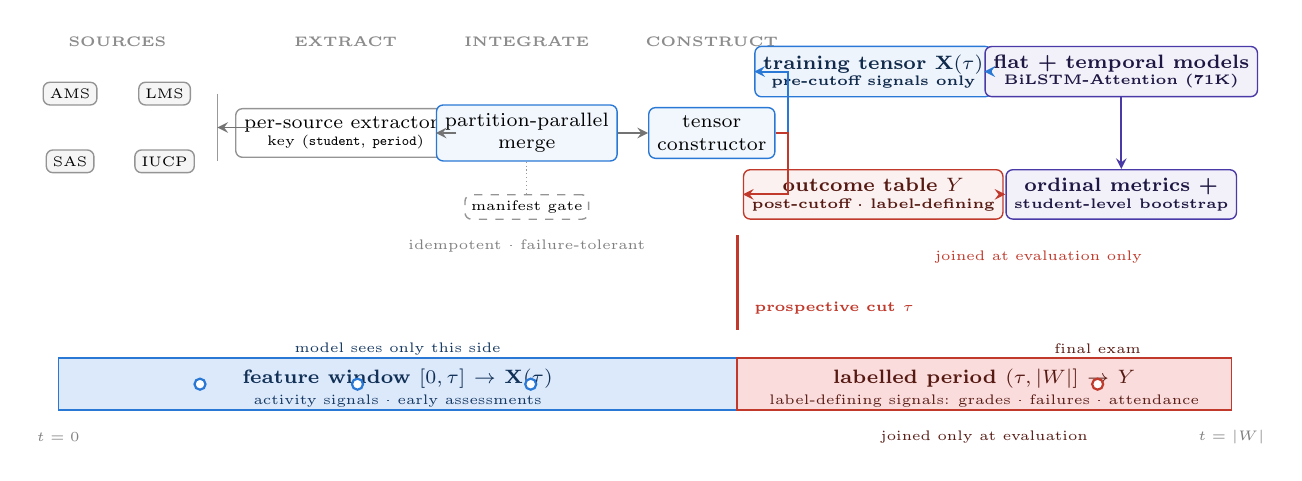
\begin{tikzpicture}[
  >={stealth},
  box/.style={draw=black!42, line width=0.5pt, rounded corners=2.4pt, align=center,
              inner sep=3.0pt, font=\scriptsize, fill=white},
  src/.style={box, fill=black!4, font=\tiny, inner sep=2.4pt},
  stage/.style={font=\tiny\bfseries, text=black!45},
  ann/.style={font=\tiny, text=black!50, align=center},
  bluebox/.style={box, draw=pipeblue, fill=pipeblue!8, text=pipeblue!35!black,
                  font=\scriptsize\bfseries, align=center},
  redbox/.style={box, draw=pipered, fill=pipered!7, text=pipered!45!black,
                 font=\scriptsize\bfseries, align=center},
  viobox/.style={box, draw=pipeviolet, fill=pipeviolet!7, text=pipeviolet!40!black,
                 font=\scriptsize\bfseries, align=center},
  flow/.style={->, line width=0.7pt, draw=black!55},
  bflow/.style={flow, draw=pipeblue},
  rflow/.style={flow, draw=pipered, dash pattern=on 2.2pt off 1.6pt},
  vflow/.style={flow, draw=pipeviolet},
]
%
% ---- row 1: pipeline -------------------------------------------------------
\node[src] (ams) at (0.55, 0.50)  {AMS};
\node[src] (lms) at (1.75, 0.50)  {LMS};
\node[src] (sas) at (0.55, -0.36) {SAS};
\node[src] (iucp) at (1.75, -0.36){IUCP};
\node[stage] at (1.15, 1.16) {SOURCES};
\draw[black!40, line width=0.6pt] (2.42, 0.50) -- (2.42, -0.36);
%
\node[box, align=center] (ext) at (4.05, 0) {per-source extractors\\[-2pt]{\tiny key (\texttt{student}, \texttt{period})}};
\node[stage] at (4.05, 1.16) {EXTRACT};
%
\node[box, align=center, fill=pipeblue!6, draw=pipeblue] (mrg) at (6.35, 0) {partition-parallel\\ merge};
\node[stage] at (6.35, 1.16) {INTEGRATE};
\node[box, dashed, inner sep=2.2pt, font=\tiny] (man) at (6.35, -0.94) {manifest gate};
\draw[densely dotted, draw=black!40] (mrg.south) -- (man.north);
\node[ann] at (6.35, -1.44) {idempotent · failure-tolerant};
%
\node[box, align=center, fill=pipeblue!6, draw=pipeblue] (con) at (8.70, 0) {tensor\\ constructor};
\node[stage] at (8.70, 1.16) {CONSTRUCT};
%
\draw[flow] (2.98, 0.07) -- (2.42, 0.07);
%
\draw[flow] (ext.east) -- (mrg.west);
\draw[flow] (mrg.east) -- (con.west);
%
% fork: constructor -> X (blue) / Y (red)
\node[bluebox] (xt) at (10.75, 0.78)  {training tensor $\mathbf{X}(\tau)$\\[-2pt]{\tiny pre-cutoff signals only}};
\node[redbox]  (yt) at (10.75, -0.78) {outcome table $Y$\\[-2pt]{\tiny post-cutoff · label-defining}};
\draw[bflow] (con.east) -- ++(0.16,0) |- (xt.west);
\draw[rflow, solid] (con.east) -- ++(0.16,0) |- (yt.west);
%
% models + evaluation
\node[viobox] (mdl) at (13.90, 0.78)  {flat + temporal models\\[-2pt]{\tiny BiLSTM-Attention (71K)}};
\node[viobox] (evl) at (13.90, -0.78) {ordinal metrics +\\[-2pt]{\tiny student-level bootstrap}};
\draw[bflow] (xt.east) -- (mdl.west);
\draw[vflow] (mdl.south) -- (evl.north);
\draw[rflow] (yt.east) -- (evl.west);
\node[ann, text=pipered] at (12.85, -1.58) {joined at evaluation only};
%
% ---- the cut: one red line from the fork down into the timeline ------------
\draw[pipered, line width=1.1pt] (9.02, -1.30) -- (9.02, -2.50);
\node[font=\tiny\bfseries, text=pipered, anchor=south west] at (9.12, -2.42) {prospective cut $\tau$};
%
% ---- row 2: timeline -------------------------------------------------------
\fill[winblue, draw=pipeblue, line width=0.5pt]  (0.40, -3.52) rectangle (9.02, -2.86);
\fill[winred,  draw=pipered, line width=0.5pt] (9.02, -3.52) rectangle (15.30, -2.86);
\node[font=\scriptsize\bfseries, text=pipeblue!40!black] at (4.71, -3.12)
  {feature window $[0,\tau]$ $\rightarrow$ $\mathbf{X}(\tau)$};
\node[font=\scriptsize\bfseries, text=pipered!45!black] at (12.16, -3.12)
  {labelled period $(\tau,|W|]$ $\rightarrow$ $Y$};
\node[ann, text=pipeblue!45!black] at (4.71, -3.40) {activity signals · early assessments};
\node[ann, text=pipered!45!black] at (12.16, -3.40) {label-defining signals: grades · failures · attendance};
%
\foreach \x in {2.2, 4.2, 6.4}{
  \draw[pipeblue, line width=0.8pt, fill=white] (\x, -3.19) circle (0.07);
}
\draw[pipered, line width=0.8pt, fill=white] (13.6, -3.19) circle (0.07);
\node[ann, text=pipered!45!black] at (13.6, -2.74) {final exam};
\node[ann, text=pipeblue!45!black] at (4.71, -2.74) {model sees only this side};
\node[ann] at (0.40, -3.86) {$t=0$};
\node[ann] at (15.30, -3.86) {$t=|W|$};
\node[ann, text=pipered!45!black] at (12.16, -3.86) {joined only at evaluation};
%
\end{tikzpicture}
